%=======================+=========================
%================  Simulation  ================
%=================================================
\section[Monte Carlo]{Monte Carlo simulation \label{sec:simulation}}
The detailed simulation of events in the Hall-D beam line and GlueX detector is performed with a Geant-based simulation.The package was originally developed within the GEANT3 framework~\cite{Brun:1987ma} and recently migrated to the GEANT4 framework~\cite{Agostinelli:2002hh,Allison:2016lfl}. The simulation framework uses the same geometry definitions and magnetic field maps as used in reconstruction and is able to simulate the primary photon beam from the bremsstrahlung radiator through the GlueX detector to the photon beam dump, as well as doing event simulations of photoproduction events in the GlueX detector itself. The simulation broadly follows the diagram as shown in Fig.~\ref{fig:MC-data-flow}. Events of interest are generated using either a predefined or user-supplied event generator. The events are read in by the Geant-based Hall-D Monte Carlo, which obtains the appropriate geometry and magnetic field information from the geometry and calibration data bases. The resulting events are then processed by a digitization package. This package obtains run-dependent information from both the calibration and run-conditions data bases and background events from a file. The simulated events have appropriate inefficiencies applied, and then together with the background events, are digitized to look like raw data from the experiment. The resulting events are then processed with same reconstruction software as used for the real events and the output is saved to a REST file. These files are then made available for physics analysis.
\begin{figure}[h!]\centering
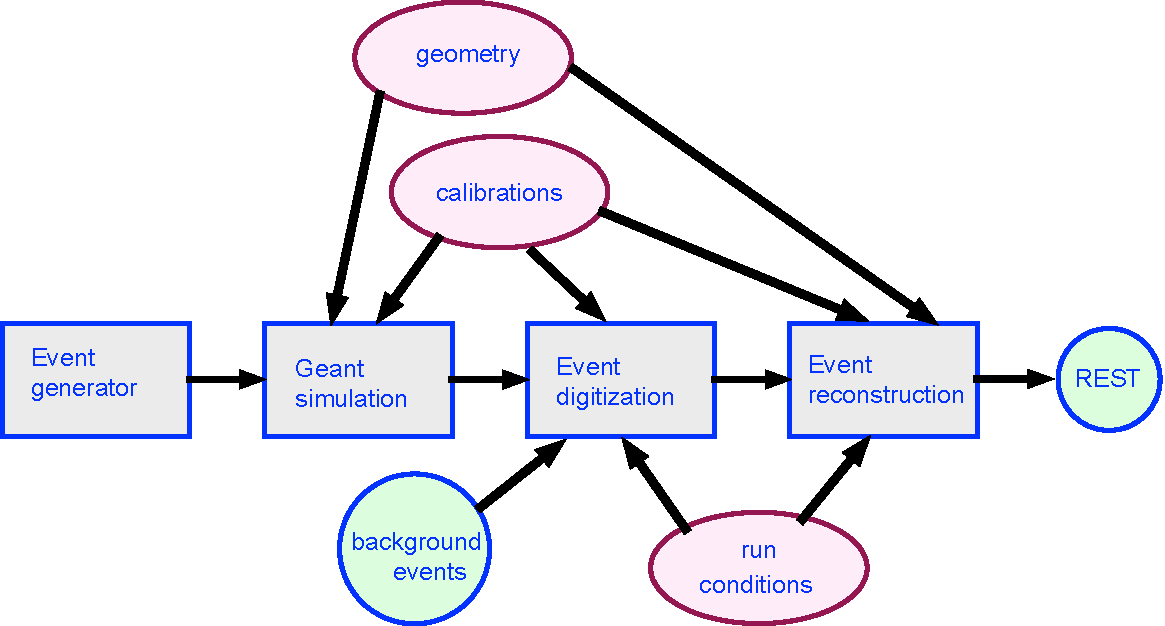
\includegraphics[width=0.85\textwidth]{figures/MC-data-flow.pdf}
\caption[]{\label{fig:MC-data-flow}The data flow from event generator through physics analysis files for Monte Carlo events.}
\end{figure}
\subsubsection[Material thickness]{\label{sec:materialscan}Geometry definitions}
The geometry and material descriptions for the experiment are common across simulation and reconstruction. The primary description resides in a family of xml files which all follow a common dtd or schema called the Hall D Detector Specification, or HDDS \textcolor{blue}{CITATION??}. Run-specific variations to this description are maintained in the Calibration Database, including information on missing and problematic electronic channels. The common magnetic field map is also maintained in the calibration database.

\subsection{Event generators \label{sec:generators}}
Simulation starts with the generation of events, which can be specific particles or reactions, or a background generator. A common tool set has been developed to minimize redundancy in code. These tools include standard methods to generate the distributions of primary photon beam energies and polarization. An output interface to produce files suitable as input for Geant simulation.

The photon beam energy distribution can be produced using a coherent bremsstrahlung generator that accounts for the physical properties of the radiator and the photon beamline.This generator also allows the user to select the orientation of the diamond radiator and then calculates the linear polarization for each photon. Photons can also be generated according to the spectrum measured in the pair spectrometer during any actual data run by interfacing to the calibration data base. In this method, the user inputs the degree of linear polarization and the orientation. Finally, the user can provide a histogram of the photon energy spectrum and a second one of the degree of polarization that is used to generate the photon beam. 

One of the first generators has been used to simulate the entire photoproduction cross section and is used to study backgrounds to physics reactions as well as develop analysis tools for extracting signals. This is based on Pythia~\cite{Sjostrand:2006za}, but includes additions that describe the low-energy photoproduction cross sections. Other generators are tied to specific reactions, where the generator needs to describe the underlying physics

\subsection{HDGeant \label{sec:hdgeant}}
As noted earlier, both Geant3 and Geant4 versions are available for simulation of the experiment. Both versions have been tuned to reproduce the behavior of the experiment, but there are some differences due to differences in how the two versions of Geant decide when to stop tracking particles. In general, simulation is carried to mimic the running conditions found across a range of runs; typically a large part of a single run period. The output from Geant is both hit time and energy deposits in detector volumes. 

\subsection[mcsmear]{Detector Response}
Converting the time and energy deposits coming from Geant into electronic detector responses that match what is readout from the experiment is carried out by the detector response package (mcsmear). The output of this digitization is identical to the real data with the exception that the so-called \emph{truth information} about the data is retained to allow detailed performance studies. In addition to the digitization, it is at this stage that run-dependent efficiency effects are applied to the data. This includes both missing electronic channels, as well as reduced efficiency of other channels. Additional smearing of some signals is also applied here to better match the performance of the Monte Carlo to data. 

In addition to the digitization, this package also folds measured backgrounds into the data stream. During regular data collection, random triggers are collected on a regular basis during each run. These are separated from the actual data and used to provide experimental background signals in the Monte Carlo, with rate of random events added based on the actual beam fluxes in the experiment. 

\subsection{Job submission \label{sec:jobsubmission}}
Because of the large number of experimental conditions that need to be matched in simulating data, the \emph{MCWrapper} tool has been developed to manage simulations. Users who need a Monte Carlo sample use a web-based interface to MCWrapper to select the event generator, the version of Geant, the run period of interest and versions of reconstruction code. MCWrapper then assembles the correct information and submits the needed simulation and reconstruction jobs to the Open Science Grid. Once the jobs are completed, the user has access to the reconstructed event sample.